\documentclass[a4paper]{article}

\usepackage{INTERSPEECH2021}
\usepackage{subfiles}
\usepackage{datatool}
\usepackage{fmtcount}
\usepackage{xstring}
\usepackage{substr} % Include this in your preamble
\usepackage{tipa}
\DTLloaddb{cronbach}{scripts/data_output/cronbach_alpha.csv}
\DTLloaddb{modelsouts}{scripts/data_output/dynamic_models.csv}
\DTLloaddb{partrem}{scripts/data_output/participant_removal.csv}
\DTLloaddb{taskrem}{scripts/data_output/taskremoval.csv}

\newcommand{\livedata}[2]{%
    \DTLfetch{#1}{Statistic}{#2}{Value}%
}

\title{Measuring music and prosody: accounting for variation in non-native speech discrimination with L1, L2, music skills, and working memory}
%Paper submission must be anonymous. Only fill in author information for the final PDF.
\name{Author Anonymous$^1$, 
Co-author Anonymous$^1$,
Co-author Anonymous$^1$,
Co-author Anonymous$^1$}
%The maximum number of authors in the author list is twenty. If the number of contributing authors is more than twenty, they should be listed in a footnote or in acknowledgement section, as appropriate.
\address{
  $^1$Author Affiliation}
\email{author@university.edu, 
coauthor@company.com}

\begin{document}

\maketitle
% 
\begin{abstract}
The dynamics of non-native speech perception remain poorly understood, especially in accounting for specialized skills/training. One such skill, musical ability, has been shown to positively impact sensitivity to speech sounds, yet how musical ability is operationalized and measured varies from study to study. Individuals’ musical abilities vary in exposure-duration, skill type (e.g., voice, percussion), and skill-level. Here, we take an individual differences (n=\livedata{partrem}{kept_participants}) approach to explore sensitivity in non-native speech discrimination of prosodic contrasts. We measure language background, general cognitive measures, and three measures of musical ability: auditory-motor temporal integration \cite{Kachlicka_Saito_Tierney_2019}, auditory discrimination \cite[MET]{Wallentin_Nielsen_Friis-Olivarius_Vuust_Vuust_2010}), and musical sophistication \cite[Goldsmiths-MSI]{Müllensiefen_Gingras_Musil_Stewart_2014}. We measured prosodic sensitivity using three AX discrimination tasks and signal detection measures (d'): Mandarin tone (primarily cued by pitch), Italian and Japanese (non-)geminates (primarily cued by duration). Results suggest music background, discrimination, and auditory-motor temporal integration capture related –yet divergent– aspects of music experience. Additionally, music sub-skills (e.g., pitch perception) have unequal contributions to non-native speech sensitivity across languages' respective linguistic cues (e.g., tone). Findings support models of non-native speech perception, which consider cognitive factors and auditory experience outside of language experience.

\end{abstract}
\noindent\textbf{Index Terms}:  Individual differences, Music, Non-native speech perception, Measuring prosody
\section{Introduction}

Non-native speech perception is complex, with many speech contrasts causing difficulties for beginner L2 learners (e.g., \cite{Flege_95}). For example, Italian and Japanese learners often struggle to differentiate between geminate and non-geminate contrasts (e.g., Japanese /kate/ \textit{win}, geminate /kat:e/ \textit{buying}; Italian /\textipa{Eko}/ \textit{echo}, geminate /\textipa{Ek\textlengthmark o}/ \textit{here}). Similarly, Mandarin learners struggle to distinguish between the different tones of Mandarin (Tone 1 high flat, Tone 2 rising, Tone 3 low falling-rising, Tone 4 falling)\cite{Pelzl_2021}. Whereas non-native speech contrasts are difficult for most people, it has long been understood that some individuals come to the task of L2 learning with an advantage, evidenced by the fact that two people studying for the same duration have variant language proficiency across language sub-skills \cite{Zheng_2021}. Further, within speech perception L2 learners vary substantially in how well they are able to distinguish non-native speech contrasts from the onset of learning.

One of the most studied areas of individual differences in non-native speech perception comes from the study of L1 transfer effects. Amongst other models, the Perceptual Assimilation Model and Speech Learning Model both successfully demonstrate how a learner’s L1 influences L2 non-native speech perception and learning \cite{Flege_95,Best_1995}. A second but related line of research suggests that individual cues used to discriminate non-native speech contrasts have a major impact on a learner's ability to acquire speech sounds, particularly true for prosodic cues found in geminate and tonal contrasts. For example, \cite{Francis_2008} suggests that tone experience in the L1 improves L2 discrimination.
Similarly, Japanese speakers start off with 80\% accuracy in Italian geminate discrimination \cite{Tsukada_Cox_Hajek_Hirata_2017}. Further, \cite{Pajak_2014} shows that both duration and siblant sensitivity transfers in a gradient manner as a function of how much the respective cues is in the L1, regardless of where the cue occurs in the language. 

More recently, this same line of research has looked beyond cues similarities in L1 and L2 by examining the role of music training on L2 speech perception. The rationalization, here, is that linguistic and musical cues often share the same acoustic correlates, e.g., F0 and duration. For example, \cite{Wiener_Bradley_2020} demonstrates how short term focused musical pitch training is as beneficial for Mandarin tone discrimination as classroom learning. Beyond this, general musical skills/aptitude and even general cognitive abilities (e.g., \cite{Zheng_2021}) have both been linked to and disputed as successful predictors of improved non-native speech perception. For example, \cite{Zheng_2021} suggests that music aptitude is only weakly predictive of variation in non-native speech perception, whereas general cognitive acoustic abilities are more reliable. This is in contrasts to \cite{Slevc_2006}, which finds that musical ability is strongly tied to speech level language abilities. 

These seemingly contradictory results suggest a need for a more nuanced approach to understanding the relationship between individual differences (particularly in music subskills) and non-native speech discrimination abilities. In the current study, we investigate the ways in which different aspects of musical experience affect non-native speech perception by operationalizing music experience in three ways: productive measures (auditory-motor temporal integration) \cite{Kachlicka_Saito_Tierney_2019}, perceptual measures (auditory discrimination) \cite[MET]{Wallentin_Nielsen_Friis-Olivarius_Vuust_Vuust_2010}), and musical sophistication \cite[Goldsmiths-MSI]{Müllensiefen_Gingras_Musil_Stewart_2014}. Both modalities of music measurements (productive and perceptual) test pitch and rhythm abilities, separately. Beyond music, we use a digit span task as a measure of working memory. Lastly, we measure linguistic sensitivity and experience through three AX discrimination tasks (i.e., Italian and Japanese geminate contrasts, Mandarin tone contrasts) and language questionnaire, respectively. Italian, Japanese, and Mandarin were chosen because of their direct link to music acoustic dimensions (i.e., duration and F0).

Based on the previous review, the following research questions were formulated: 1) To what extent do various measures of musical experience and skill predict non-native speech sensitivity in Italian, Japanese, and Mandarin? To answer this question, we look at how different modalities and dimensions of musical measures predict linguistic sensitivity across Italian, Japanese, and Mandarin. 2) To what extent does language experience deferentially predict non-native speech sensitivity in Italian, Japanese, and Mandarin? To answer this, we examine the role of the L1 and L2 in respects to each language task. 3) To what extent do domain general cognitive abilities deferentially predict non-native speech sensitivity in Italian, Japanese, and Mandarin? To answer this, we examine the role of working memory in each language task.

\section{Methods}

\subsection{Participants}
 The recruitment of \livedata{partrem}{starting_participants} English Native speakers was managed through Prolific \cite{Palan_2018} (n=\livedata{partrem}{data_exp_142778-v2.before})  and in-person (n=\livedata{partrem}{data_exp_141883-v12.before}) recruitment. In person recruitment was done in both music and language classrooms, meaning many participants have both language and music experience. Additionally, 22 potentional participants were rejected from participation due to failing initial requirements (i.e., eight removed for failed headphone-check \cite{milne_2021} and 14 removed for eye-tracking calibration failure, which is not reported here). To ensure data quality and maximize retained participants, three median absolute deviations (MAD) from median score was calculated as the standard for removal for each task \cite{Leys_2013}. Of the \livedata{partrem}{starting_participants} participants who remained, \livedata{partrem}{removed_participants} were removed for low accuracy scores. Of these, \livedata{taskrem}{particip_remove_lang.remove} were removed for being below MAD range in the language tasks and \livedata{taskrem}{rhythm_part.remove} removed for low performance in auditory-motor integration task.  After removal, \livedata{partrem}{kept_participants} participants' (age: $\mu$ = \livedata{partrem}{mean_age}, $\sigma$ = \livedata{partrem}{sd_age}) data were retained for analysis. 

\subsection{Procedure}
All of the participants took part in a multi-stage battery of language, music, and domain general tasks.\footnote{Gorilla experiments, R scripts, and data are all available through the OSF link: https://osf.io/bsph6/?view_only=28ea5c350d8b4c75868ac26f4e35e5d2} Participants first took part in a headphone check (dichotic-pitch task) \cite{milne_2021}, followed by an 8 trial adaptive staircase digit-span task. After completing the head-phone check and digit-span tasks,
all participants took part in either music or language segments, followed by the complementary segment (i.e., music $\rightarrow$ language, language $\rightarrow$ music). For all language and music tasks, stimuli and experimental design were adapted and built in Gorilla \cite{gorilla_Anwyl-Irvine_2019} for the current study from previous in-person studies (e.g., Mandarin \cite{Wiener_Bradley_2020}) that either made materials openly available on OSF \cite{OSF} or were provided by the original authors. 

In the language segment, participants took part in three speeded AX-discrimination tasks for Italian, Japanese, and Mandarin (trials automatically proceeded after 1000 ms)\cite{Hayes‐Harb_Barrios_2021}. All Language stimuli were sampled at 44.1 kHz and recorded in sound attenuated booths (Mandarin) or a studio (Japanese and Italian). The Italian and Japanese AX tasks, adapted from \cite{Tsukada_Cox_Hajek_Hirata_2017}, consisted of stop geminate contrasts: Italian - /\textipa{p t k b d g dZ}/, Japanese - /\textipa{t k tS}/. For the Italian AX task, stimuli consisted of 27 pairs of geminate contrasts (e.g., non-geminate /\textipa{Eko}/ \textit{echo}, geminate /\textipa{Ek\textlengthmark o}/ \textit{here}), which were made up of approximately half real and non-real words, spoken by three native speakers. For the Japanese AX task, stimuli consisted of 33 pairs of geminate contrasts, with approximately half of the geminate and non-geminate pairs matching in pitch-accent (e.g., non- geminate low-high pitch-accent /heta/ \textit{unskilled}, geminate low-high pitch-accent /het:a/ \textit{decreased}) and mismatching in pitch-accent (e.g., non-geminate high-low pitch-accent /kate/ \textit{win}, geminate low-high pitch-accent /kat:e/ \textit{buying}). The Mandarin task, adapted from \cite{Wiener_Bradley_2020}, consisted of 8 stimuli based on the Mandarin Pinyin syllable yu with four tones (yu1, yu2, yu3, yu4) recorded by male and female native speakers and were normalized for F0 manipulation using \cite{Boersma_Weenink}'s method. Each tonal pairing co-occurred equal amounts with each tone occurring with itself three times to equalize match-mismatch answers across the task. 

The music segment has two basic tasks: auditory-motor temporal integration \cite{Kachlicka_Saito_Tierney_2019} and auditory discrimination \cite[Musical Ear Task]{Wallentin_Nielsen_Friis-Olivarius_Vuust_Vuust_2010}, both of which have melody and rhythm sections. In the auditory-motor integration tasks, participants hear a rhythm (auditory-motor rhythm) or melody (auditory-motor melody) three times, memorizes it, and reproduces either the melodic or rhythmic phrase. For example, in the auditory-motor rhythm task each trial plays a 13 beat rhythm three times. The participant then needs needs to repeat the exact beat using the space-bar. Timing is captured on each space-bar press. Similarly, for the auditory-motor melody task a series of 7 notes are played, the participants then needs to repeat these with a series of on-screen buttons that correspond to relative pitches (always starts with the middle pitch). After completion of both auditory-motor temporal integration tasks, the participant then does a rhythm and melody Musical Ear Task. \cite{Wallentin_Nielsen_Friis-Olivarius_Vuust_Vuust_2010}, where two auditory music samples (melody or rhythm) are played then participants must determine if the samples were identical (melodies or drum beats) through a button press on the screen. 

After completing the music and language segments, participants then fill in both a musical sophistication survey \cite[Goldsmiths-MSI]{Müllensiefen_Gingras_Musil_Stewart_2014} and a Language Experience and Proficiency Questionnaire (LEAP-Q) \cite{Marian_Blumenfeld_Kaushanskaya_2007}. The Goldsmiths-MSI is a self-reported survey, which aims to capture individual differences through musical sophistication in 5 areas: Active Musical Engagement (e.g., time and money resources spent on music); Self-reported Perceptual Abilities (e.g., musical listening skills); Musical Training (e.g. formal musical training); Self-reported Singing Abilities (e.g. one’s own singing); Emotional Engagement with Music (e.g. ability to talk about emotions in music). Finally, the participant fills out the LEAP-Q with self-reported data on their language proficiency and experience of bilingual and multilingual practices. 

\subsection{Data Analysis}
\subsubsection{Data Wrangling and Validation}


Reaction time based data removal was calculated by overall trial log transformed reaction time on both the Musical Ear Tasks (rhythm and melody). MAD was used as the removal standard, reaction time trial data outside three deviations was removed (proportion of trials removed from musical ear tasks: \livedata{taskrem}{RTmet.remove} of \livedata{taskrem}{RTmet.before} trials). Language tasks reaction time were squareroot transformed, but no trail data was removed due to the automatic progression of trials at 1000ms.

Data removal based on accuracy was then calculated by item for both Musical Ear Tasks and for each language task. The standard of three MADs was applied to each task's accuracy; retained items by task: Auditory-motor melody items \livedata{taskrem}{melody_item.after}/\livedata{taskrem}{melody_item.before}, Auditory-motor rhythm items \livedata{taskrem}{rhythm_item.after}/\livedata{taskrem}{rhythm_item.before}, Mandarin items \livedata{taskrem}{Mandarin.after}/\livedata{taskrem}{Mandarin.before}, Italian items \livedata{taskrem}{italian.after}/\livedata{taskrem}{italian.before}, Japanese items \livedata{taskrem}{japanese.after}/\livedata{taskrem}{japanese.before}. Additionally in the auditory-motor rhythm task, the first beat of every trial (rhythmic phrase) was removed. This was done because the first beat initiates rhythm capture. As each possible beat is 200 ms apart, the second beat of each rhythmic phrase was then centered by subtracting 100 ms, as seen in fig \ref{fig:beat_data}

\begin{figure}[t]
  \centering
  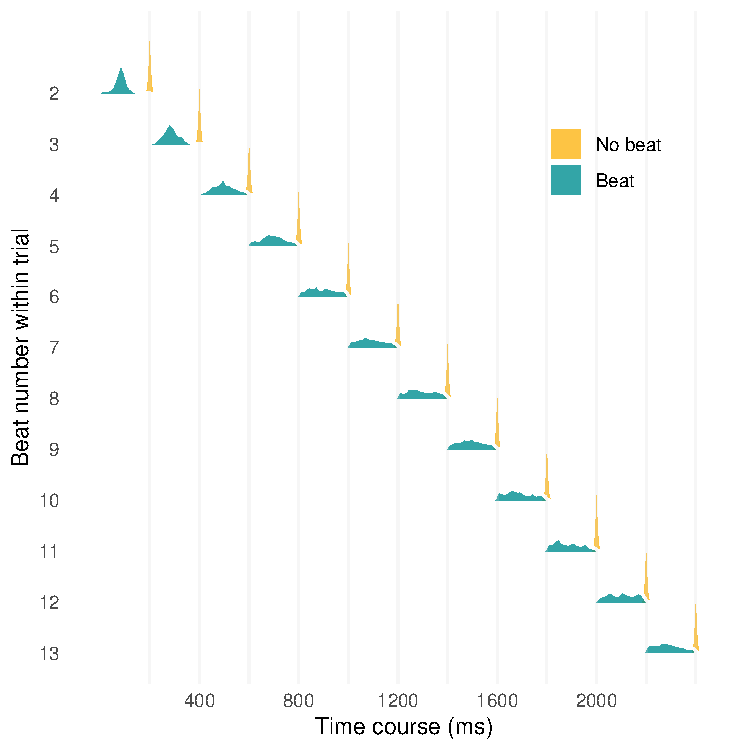
\includegraphics[width=\linewidth]{SP_24_visuals/Correct_and_Incorrect_distrubutions_by_beat_across_trial.pdf}
  \caption{distribution of beats hit (space bar) over trials. Timing frames for each of beat (2-13) is illustrated by horizontal lines. No-beat distributions represent \cite{gorilla_Anwyl-Irvine_2019}'s measurement sensitivity}
  \label{fig:beat_data}
\end{figure}

After data removal, Cronbach's alpha was calculated for each of the musical tasks and questionnaire as tested in original studies (i.e., Goldsmiths 5 area scores, \textit{Musical Ear Task} melody and rhythm items, auditory-motor melody, auditory-motor rhythm) to test internal reliability of items in each task. Results as compared to original studies are presented in Table~\ref{tab:comparison}. 

\begin{table}[ht]
\centering
\begin{tabular}{|c|c|c|}
\hline
\textbf{Task} & \textbf{Reported Value} & \textbf{Our Value} \\
\hline
GoldSmiths \cite{Müllensiefen_Gingras_Musil_Stewart_2014} & Range: 0.79 - 0.93 & 0.89 \\
Musical Ear tasks \cite{Wallentin_Nielsen_Friis-Olivarius_Vuust_Vuust_2010}& 0.87 & 0.79 \\
Auditory-motor melody \cite{Kachlicka_Saito_Tierney_2019}& Unreported & 0.93 \\
Auditory-motor rhythm\cite{Kachlicka_Saito_Tierney_2019}& Unreported & 0.91 \\
\hline
\end{tabular}
\caption{Comparison of reported Cronbach's alpha values compared to our Cronbach's alpha values}
\label{tab:comparison}
\end{table}

For both Musical Ear tasks and each language task,  D-prime (d′) was calculated as a measure of sensitivity\cite{Macmillan_Creelman_2004}. 

\subsubsection{Statistical Analysis}


All quantitative variables from each of the tasks were centered on their mean to 0 and normalized so that the scale of individual variables was similar across tasks , as seen in figure \ref{fig:centered_data}.

\begin{figure*}[t]
  \centering
  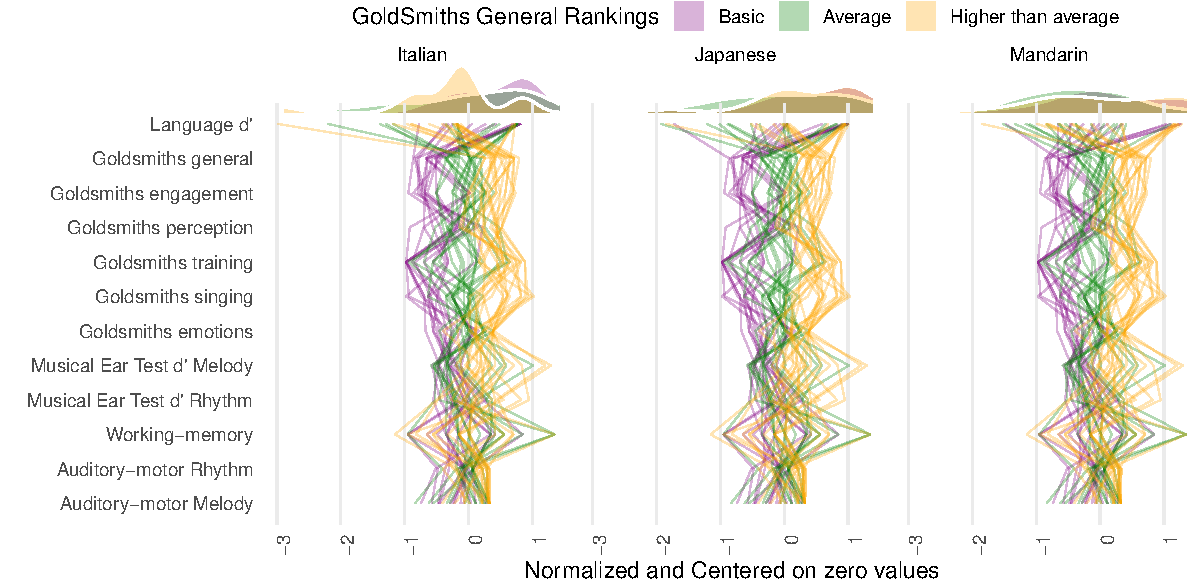
\includegraphics[width=.9\textwidth]{SP_24_visuals/by_gs.pdf}
  \caption{Raw data}
  \label{fig:centered_data}
\end{figure*}

To test how various measures of musical experience and skill, language experience, and domain general cognitive abilities differentially affect Italian and Japanese geminate contrast sensitivity and Mandarin tone sensitivity, three multiple linear regression models were built to compare the relative contribution of each task on centered d-prime scores of each language. Maximal Models were built using the \textit{lm} package \cite{lmPackage} in R \cite{RManual}. Each model included 14 predictor effects: L1 (coded as match no match), L2 (coded as match no match), Music student (coded as does or does not actively play an instrument/sing), Goldsmiths general, Goldsmiths engagement, Goldsmiths perception, Goldsmiths training, Goldsmiths singing, Goldsmiths emotions, Musical Ear Test d' Melody, Musical Ear Test d' Rhythm, Working-memory, Auditory-motor Rhythm, Auditory-motor Melody). Models were reduced in the following order: removal of non theoretical driven music skill (e.g., rhythm for Mandarin and Melody for Italian and Japanese), then effects were removed based on how much variance was explained in terms of coefficients and post hoc colinearity. Japanese and Mandarin models, were reduced minimally due to finding early evidence of parsimonious models. For Italian, the model was reduced until all co-linearity was no longer apparent. 

\section{Results}
Results from the Italian linear model found significant effects for: GoldSmiths general ($\beta$ = \livedata{modelsouts}{Italian.gs_general.estimate}, \text{SE} = \livedata{modelsouts}{Italian.gs_general.std.error}, z = \livedata{modelsouts}{Italian.gs_general.statistic}, p \textless{} \livedata{modelsouts}{Italian.gs_general.p.value}), indicating that higher musical general self ratings predict lower sensitivity to Italian geminate contrasts; Working memory ($\beta$ = \livedata{modelsouts}{Italian.mean_working_memory.estimate}, \text{SE} = \livedata{modelsouts}{Italian.mean_working_memory.std.error}, z = \livedata{modelsouts}{Italian.mean_working_memory.statistic}, p \textless{} \livedata{modelsouts}{Italian.mean_working_memory.p.value}), indicating that higher working memory capacity predicts better ability to attenuate to sensitivity needed for Italian geminate contrasts.

Results from the Japanese linear model found significant effects for: GoldSmiths active engagement ($\beta$ = \livedata{modelsouts}{Japanese.gs_activeeng.estimate}, \text{SE} = \livedata{modelsouts}{Japanese.gs_activeeng.std.error}, z = \livedata{modelsouts}{Japanese.gs_activeeng.statistic}, p \textless{} \livedata{modelsouts}{Japanese.gs_activeeng.p.value}), indicating that higher amounts of musical engagement predict lower sensitivity to Japanese geminate contrasts; Goldsmiths Singing ability ($\beta$ = \livedata{modelsouts}{Japanese.gs_singingabil.estimate}, \text{SE} = \livedata{modelsouts}{Japanese.gs_singingabil_memory.std.error}, z = \livedata{modelsouts}{Japanese.gs_singingabil.statistic}, p \textless{} \livedata{modelsouts}{Japanese.gs_singingabil.p.value}), indicating that higher self ratings in music singing ability predicts higher sensitivity for Japanese geminate contrasts. Working memory ($\beta$ = \livedata{modelsouts}{Japanese.mean_working_memory.estimate}, \text{SE} = \livedata{modelsouts}{Japanese.mean_working_memory.std.error}, z = \livedata{modelsouts}{Japanese.mean_working_memory.statistic}, p \textless{} \livedata{modelsouts}{Japanese.mean_working_memory.p.value}), indicating that higher working memory capacity predicts better ability to attenuate to sensitivity needed for Japanese geminate contrasts;
Auditory-motor Rhythm ($\beta$ = \livedata{modelsouts}{Japanese.beat_score.estimate}, \text{SE} = \livedata{modelsouts}{Japanese.beat_score.std.error}, z = \livedata{modelsouts}{Japanese.beat_score.statistic}, p \textless{} \livedata{modelsouts}{Japanese.beat_score.p.value}), indicating that higher productive rhythmic ability predicts greater sensitivity to Japanese geminate contrasts.

Results from the Mandarin linear model found significant effects for: GoldSmiths emotions ($\beta$ = \livedata{modelsouts}{Mandarin.gs_emotions.estimate}, \text{SE} = \livedata{modelsouts}{Mandarin.gs_emotions.std.error}, z = \livedata{modelsouts}{Mandarin.gs_emotions.statistic}, p \textless{} \livedata{modelsouts}{Mandarin.gs_emotions.p.value}), indicating that higher musical emotional ratings predict lower sensitivity to Mandarin tone; Musical Ear Test melody ($\beta$ = \livedata{modelsouts}{Mandarin.MET_dprime_melody.estimate}, \text{SE} = \livedata{modelsouts}{Mandarin.MET_dprime_melody.std.error}, z = \livedata{modelsouts}{Mandarin.MET_dprime_melody.statistic}, p \textless{} \livedata{modelsouts}{Mandarin.MET_dprime_melody.p.value}), indicating that higher perceptual sensitivity to musical pitch predicts higher sensitivity to Mandarin tone. 

All model outputs can be seen in figure \ref{fig:model}. The structure of the model terms in figure \ref{fig:model} is the original maximal model structure for each language. Parsimonious Model structure is the remaining items in the visual. If a term does not have a present co-efficient it means that it was not in the parsimonious model of that language.

\begin{figure}[t]
  \centering
  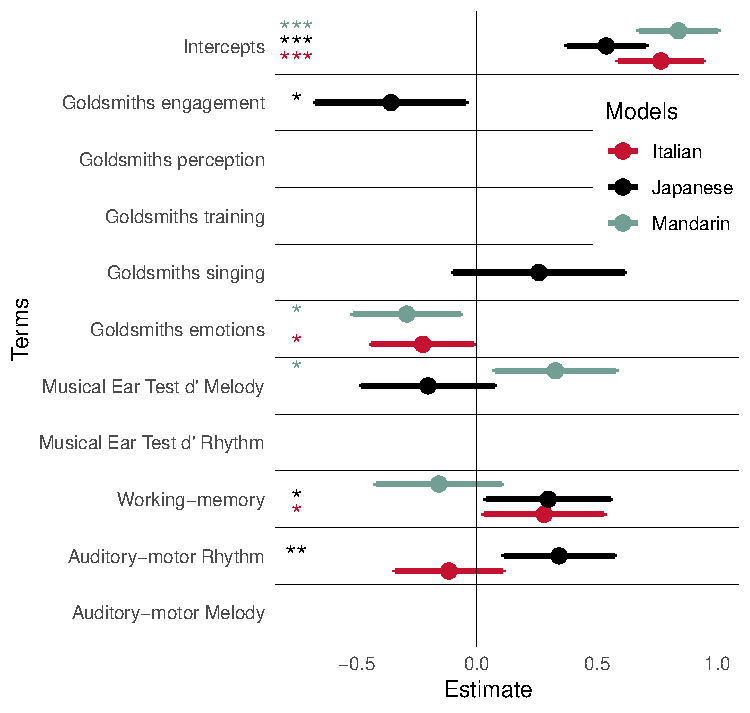
\includegraphics[width=\linewidth]{SP_24_visuals/Japanese,Italian,_Mandarin_max_models_structure:_parsimonious_effects.pdf}
  \caption{Each language's parsimonious model output}
  \label{fig:model}
\end{figure}

\section{Discussion}

The popular conjecture that musical ability is associated with L2 proficiency is not a myth \cite{Slevc_Miyake_2006b}, however, the relationship is not straightforward in that language sensitivity is positively predicted by cue dependent and modality specific measure of music ability. For example, musical pitch perceptual abilities do indeed predict Mandarin tone sensitivity. Interestingly, however, this does not carry over to the motor-auditory melody task, suggesting that the ability to productively recreate the pitches from that motor-auditory task does not have a direct relationship with the ability to perceive differences between Mandarin tones. In contrast, Japanese model results suggest that rhythm ability is indeed tied to Japanese geminate perception. However, only motor-auditory rhythmic ability has this relationship for sensitivity to Japanese geminate contrasts. Surprisingly, this does not carry over to the Italian task. It could be that the difference between Mandarin and Japanese model results have to do with how direct the relationship is between the linguistic cue and the musical cue. In the case of Mandarin tones and musical pitch, the same underlying cue is used for discrimination of both (i.e., F0), whereas the relationship between geminate contrasts and music rhythm is less clear. While both use duration cues for discrimination, music rhythm, in our tasks, is measured as the ability to attenuate to the time between beats or the inter-beat interval, while geminate contrasts often rely on the duration of a consonant. In the case of Italian, It could be that no relationship between rhythm and language sensitivity was found because of the changes in vocalic pronunciation between geminate and non-geminate contrasts (co-articulation). In this way, it could be that Italian sensitivity would be better predicted by a persons ability to discriminate or produce formant differences. 

While specialized skills in music are indeed positively predictive of non-native speech sensitivity, musical self reported measures have the opposite effect with the exception of higher singing ability predicting better Japanese discrimination. That is, in all cases (besides singing ability) throughout the models of each language, higher Goldsmith music sophistication scores predict lower non-native speech sensitivity. As seen in figure \ref{fig:centered_data}, Goldsmiths score are highly correlated. This could be due to the fact that our population has a high proportion of professional musicians. However, the results do suggest that higher music self ratings predict lower language sensitivity.    

In terms of research question 2, language experience in either the L1 or L2 has little effect on a persons ability to discriminate speech contrasts across the models. However, this may be due to the fact that our recruitment gathered mostly English L1 speakers and had many more people that do not have experience with each of these languages than those that do. This is partially unavoidable since we are recruiting multiple languages and very few people are studying Mandarin, Japanese, and Italian simultaneously or even a combination of any two of these languages. Sensitivity results in figure \ref{fig:dprime} suggest that those that have experience with a language do indeed have a greater sensitivity to the language, even outperforming those with musical experience in many cases. 

Lastly, both the Japanese and Italian model suggest that working memory is a crucial predictor for sensitivity to geminate contrasts. However, the Mandarin model does not. This could be due to the fact that Mandarin words in our task are single syllable words, and Japanese and Italian words are multiple syllable words. Further, this result could be due to the dimensionality of tone and geminate contrasts. Unlike tone, which has continuous cues for discrimination throughout a word, geminate contrasts happen only in limited segments of Japanese and Italian words. This could mean that partial information in the Mandarin task is sufficient, but higher cognitive demand is necessary for the Japanese and Italian tasks.

\section{Conclusions}

The dynamics of non-native speech perception are complex. However, the skills and background that predict greater sensitivity in different languages are cue-specific and modality-dependent. Music skills' positive impact for language skills does not carry over to self-rated tasks in which participants give themselves scores. While language experience does not seem to make a difference in terms of linguistic sensitivity, the importance of working memory is language-dependent. Together, these findings suggest that the relationship between music skills and experience and language skills is complex and demands future investigations. Crucially, however, music skill must have a direct linguistic cue correlate for the skill to matter. These findings support models of non-native speech perception, which consider cognitive factors and auditory experience outside of language experience.

\section{Acknowledgements}

We would like to thank XXXX funding this project and the language instructors that allowed us to recruit in their classrooms

\bibliographystyle{IEEEtran}
\bibliography{my_references.bib}
\end{document}
